\documentclass[12pt,letterpaper]{article}
\usepackage{natbib}

%Packages
\usepackage{textcomp}
\usepackage{fullpage}
\usepackage{float}
\usepackage{latexsym}
\usepackage{url}
\usepackage{epsfig}
\usepackage{graphicx}
\usepackage{amssymb}
\usepackage{amsmath}
\usepackage{mathtools}
\usepackage{bm}
\usepackage{array}
\usepackage[version=3]{mhchem}
\usepackage{ifthen}
\usepackage{caption}
\usepackage{hyperref}
\usepackage{amsthm}
\usepackage{amstext}
\usepackage{enumerate}
\usepackage[osf]{mathpazo}
\usepackage{dcolumn}
\usepackage{lineno}
\usepackage{pdflscape}
\usepackage{xcolor}

\usepackage{color,soul}

\DeclarePairedDelimiter\abs{\lvert}{\rvert}%
\DeclarePairedDelimiter\norm{\lVert}{\rVert}%
\newcolumntype{d}[1]{D{.}{.}{#1}}

\pagenumbering{arabic}


%Pagination style and stuff
\linespread{2}
\raggedright
\setlength{\parindent}{0.5in}
% \setcounter{secnumdepth}{0} 
% \renewcommand{\section}[1]{%
% \bigskip
% \begin{center}
% \begin{Large}
% \normalfont\scshape #1
% \medskip
% \end{Large}
% \end{center}}
% \renewcommand{\subsection}[1]{%
% \bigskip
% \begin{center}
% \begin{large}
% \normalfont\itshape #1
% \end{large}
% \end{center}}
% \renewcommand{\subsubsection}[1]{%
% \vspace{2ex}
% \noindent
% \textit{#1.}---}
% \renewcommand{\tableofcontents}{}
%\bibpunct{(}{)}{;}{a}{}{,}

%---------------------------------------------
%
%       START
%
%---------------------------------------------

\begin{document}

\section{Response to Referees}

\subsection{Referee: 1}
\noindent Concerning the section on disparity through time, perhaps hyphens should be removed; also, it may be misleading to use them, as sometimes the disparity-through-time phrase refers, in abbreviated format, to what is otherwise known (in full) as "mean relative subclade disparity through time", implemented in the DTT function in geiger.

\textcolor{blue}{We have removed hyphens from ``disparity-through-time''}

\noindent At the beginning of page 7, I am not convinced that "synapomorphies will naturally lead an apparent shift or increase in disparity when new clades appear" in all cases. This very much depends on character-state distribution and, given a sufficient number of unique traits or combinations thereof across the sample, you may have comparable levels of disparity.

\textcolor{blue}{We changed the sentence to:}

\textit{especially as synapomorphies can lead to apparent shift or increase in disparity when new clade appear (especially if the character-state distribution is skewed towards a particular clade).} l.@@@

\noindent On page 8, just to avoid confusion, PCO can also applied to quantitative data ONLY. End of page 8/beginning of page 9 could do with a small (few lines) exposition of protocols for axis selection.

\textcolor{blue}{We've added the precision for the PCO with quantitative data:}

\textit{or quantitative, or both} l.@@@

\textcolor{blue}{And added a brief mention of protocols for axis selection:}

\textit{(either by manually selecting the d axes that encompasses the desired variance or using methods such as the broken stick model; Legendre \& Legendre 2012 p.410)} l.@@@ + change cite to number

\noindent Lines 211-213 are problematic. Do the authors mean that categorical data are ALWAYS more problematic because of the listed reasons? Some remedies at least exist for euclideanarity.

\textcolor{blue}{We've now added a reference to the Cailliez (1983) correction to remedy for euclideanatrity}:

\textit{although this can sometimes be corrected, Cailliez 1983} l.@@@

\noindent Line 269, about PERMANOVA, puzzles me. Yes, the test is used, but for geometric morphometric analyses at least, other tests have been devised.

\textcolor{blue}{We have added mentions to other tests common in morphological disparity analyses:}

\textit{The last decade has also seen a series of development based on this test (e.g. the linear regression for multidimensional data Collyer et al 2015; or the phylogenetic ANOVA Adams 2014; but see Adams \& Collyer 2018; Lloyd 2016 for more).
It is worth noting that most of these test do not require the morphospace to be ordinated (see section 1 above).
Regardless of the statistical test used, they should be employed that are tailored to the question at hand, rather than simply following common practices.} l.@@@

\subsection{Referee: 2}

\noindent That said, my biggest issue was the specific way the paper was subdivided. The "Measuring..", "Testing.." and "Phylogeny" subsections seemed a bit jumbled. For instance, a lot of the best advice on designing a custom test for your data is in the "Measuring.." section. Meanwhile, the "Testing.." section is very effective at convincing the reader not to take bootstrap values literally (a good thing to be effective at!) but doesn't contain much else in the way of advice or guidance.

\textcolor{blue}{We've added some references to specific tests and insisted throughout the section that it is important to chose the right statistical test according to the data and question at hand (and pointed out to some general reviews detailing some of the options - see response to reviewer 1 above and response to specific comments below).}
% TG: Not sure if that's enough but lacking inspiration for now

\noindent The "Phylogeny" section makes no explicit reference to the models of trait evolution that exist. Ancestral state estimates are mentioned, but the potential pitfalls of imposing a (possibly, if not likely) incorrect model of trait evolution is elided. Elsewhere in the paper the authors do an excellent job warning the reader away from just accepting default options, or doing something just because "that's the way it's done". Yet here, the reader is left without knowledge that accepting the default BM model uncritically could cause major issues with both Revell-style multivariate corrections and all ASRs.

\textcolor{blue}{We've added the following caveat to the section about ASR:}

\textit{Furthermore, phylogenetic PCA are also really dependent on the evolutionary model which can be sometimes difficult to choose (e.g. the default Brownian motion model is not always appropriate; \citealt{blomberg2020})} . l.@@@

\noindent In the first two sections, the authors reference back to the four main goals of disparity analyses they outlined. Using those four goals as a guide post for reworking the Testing and Phylogeny subsections may help improve the flow and usability of those parts.

% TG: not sure what's meant here

\noindent Last bit: I think Figure 2 should be redesigned, personally. I'm not sure to whom it is targeted. The top part's clear, but I suspect the bottom part would be opaque to those who would most benefit from reading this paper. Right now, it shows every step of every option all at once. But I think focusing in on a single complex and general concept (eg, a clear visual explanation of ordination alone, or a clear representation of distance generation, or...) would serve the paper better. 

\textcolor{blue}{We have now updated the figure to be just illustrating the path from raw data to PCA (illustrating that both can be morphospaces). We updated the caption accordingly:}

\textit{Illustration between the different morphospaces and visualisation of the same dataset (the classic ``iris'' dataset of \citealt{edgar1935irises,fisher1936use}).
Morphospaces: different mathematical representations of a morphospace. A trait matrix can be ordinated matrix (e.g. in \citealt{tyler2011detecting} - or transformed into a distance matrix \citealt{Close2015}, not represented here).
Here we consider all these matrices as being \textit{morphospaces}, i.e. objects containing all the combinations of traits and observations (albeit transformed differently).
Visualisation: different  ways to represent the morphospace in 2D.
Visualisations can use either trait plots (directly from the trait matrix); or ordination axis plots (directly from the ordinated matrix).
Note that in 2D representations, it is good practice to plot both axes on the same scale to avoid visually distorting the importance of one axis).}

\subsubsection{Specific Comments:}

\noindent Line 98: "[Disparity as a proxy for ecology] is particularly common in palaeobiology" I actually don't think this is true (at least, not in the way it is most likely to be read; see last paragraph). There are entire journals (eg, Functional Ecology) dedicated to neontological studies using variation in easily measured traits across space/time (disparity) as a proxy for changes in ecosystem functions \& species interactions (ecology). Plant physiologists in particular routinely use various measurable morphological features (stem diameters, root depth, etc) as proxies for various ecological features (e.g., aridity tolerance) and compare locations. 
Functional ecologists use different language, and rarely use the literal word "disparity", but the ideas are basically the same. The big differences I perceive are in terms of (1) how easy it is to test the reliability of the proxy and (2) how often workers even attempt to rigorously test that proxy. 
I think, especially given the specific citation here \& preceding sentence, that the authors mean something along the lines of "disparity-as-ecology is one of the primary ways paleobiologist have for investigating ecosystem function". That is, the "particularly common" is in reference to the large proportion of studies that use this approach in palaeobiology. It's just that, as-written, I think it makes this common approach sound like a "weird" palaeobiologist think.

\textcolor{blue}{We've changed the sentence mentioning disparity and ecology and palaeobiology as follows:}

\textit{It is one of the primary ways to investigate ecosystem functioning in palaeobiology when the study species (and their functional characteristics) are extinct \citep{Wainwright2005}} l.@@@

\noindent Line 150 - 158: Nothing wrong or incorrect here, but the flow of this paragraph is odd. I find it very choppy. The first sentence is a long list of problems. The second is a set of two more problems. The third is a statement that everything has problems. The above three sentences, I think, could be reworked to flow more directly attached to the main point, which is that questions need to fit their data and vice versa.

% TG: change the paragraph flow

\noindent Line 171-172: Don't need e.g. and etc. in same parenthetical

\textcolor{blue}{We removed the  ``etc.''}

\noindent Lines 175 - 177: The discussion of dimension reduction using PCO here makes me think that more discussion in this paper of the importance of choosing an appropriate distance metric might be needed. That is, it'd be a whole separate paper trying to review or describe what is or is not appropriate! But I do think it's worth further emphasizing that it's a critical methodological choice that shouldn't be taken lightly for those intending to use MDS/NMDS

\textcolor{blue}{We've added the following sentence highlighting the effect of the chosen distance metric and referring to a great paper looking at it in more details:}

\textit{Note that when using a PCO, the distance metric on which to calculate the PCO can have some significant impact on the result morphospace \citep{lehmann2019}}. l.@@@


\noindent Line 195: I think you mean explicitly "geometric morphometric data". If that's true, being explicit is, I think, better.

\textcolor{blue}{We've added the term ``geometric'' to be more explicit.}

\noindent Lines 234 - 239: This implies that a central tendency is, on its own, a measure of disparity. Below, in the discussion of the position within morphospace of a clade, I think this point is made clearer. But I think the first few sentences here should be clarified a bit. Something like "or differences in the central tendencies (mean/median/mode) of clades [or subsets to be more general]"

\textcolor{blue}{We've changed the sentence to:}

\textit{disparity indices can be used compare the spread of the distributions (e.g. the range, quantiles or variance) or the differences in the central tendencies (i.e. mean, median or mode) of groups in the morphospace.} l.@@@

%TG: point 1
\noindent Lines 263 - 289: The "Testing hypotheses..." section. I feel as though this section needs to be fleshed out. A lot of very good points are made, especially with respect to bootstrapping, but a reader will walk away from this section (1) knowing that PERMANOVA exists, (2) being a bit skeptical of bootstrap support, and (3) not much else. The last paragraph is, I think, the most important in this section, and I would recommend cutting from the other two to expand this.
%TG: point 2
The general point about tailoring analyses to your data is sound, and that does make general advice hard, but not impossible. A few clear principles or even just an explanation of "same" morphospace could be useful here. That is, up in the Measuring subsection in lines 239 - 249 the authors provide a lot of good sound advice that seems more fitting here. 

%TG: I think these two points where meant to be merged no? See my response

\textcolor{blue}{We've now added more references to explicit test (see response to comment of reviewer 1). However, to respond to this comment, we have shortened the second paragraph and highlighted the importance to thing twice about which test to apply to which dataset at the end of each paragraph to really insist on this point.}

\noindent I'm just imagining a student who reads this paper early in their project. Then later, once they have data, tries to go back to look up some best practices and misses some good tips because they were in the "Measuring..." subsection instead of the "Testing..." subsection. It may be that the subsections should simply be reworked.

% TG: note sure how to handle this without rewriting and writing a "pro tips" section? Hence my non-response below:
\textcolor{blue}{We understand the reviewer's point of view and acknowledge that some parts could be missed out by inattentive readers. However, we wrote this paper with the idea in mind to make it the least prescriptive as possible (our message after the meeting at the orgin of the paper was: ``do whatever disparity analysis you want but to it for the right reasons'') so we already had to tone down some prescriptive aspects in previous draft versions of this paper.}

\noindent Disparity \& Phylogeny section: This section is good, but perhaps overlong. Although, it doesn't discuss (what I perceive to be) the biggest problem with phylogenetic corrections to disparity analyses: the choice of trait evolution model.
That is, "correcting" an ordination by imposing a specific model (e.g., Brownian) might cause more trouble than it solves if that model is a poor fit to the data.

\textcolor{blue}{We've added a caveat to this section (see main comments above).}

\noindent This is especially relevant as the discussion of Ancestral state estimation, which is entirely reliant on the model of trait reconstruction (as is briefly noted in line 315).

\textcolor{blue}{We've added the following to insist on the model part:}

\textit{All ancestral state estimates are highly dependent on the data and method used (especially which evolutionary model) [60].} l.@@@


%Running head
\begin{flushright}
Version dated: \today
\end{flushright}

\medskip
\begin{center}
\noindent{\Large \bf Disparities in the analysis of morphological disparity}
\bigskip

Thomas Guillerme$^{1,18,*, +}$,
Natalie Cooper$^{2, +}$,
Stephen L. Brusatte$^{3}$,
Katie E. Davis$^{4}$,
Andrew L. Jackson$^{5}$,
Sylvain Gerber$^{6}$,
Anjali Goswami$^{2}$,
Kevin Healy$^{7}$,
Melanie J. Hopkins$^{8}$,
Marc E. H. Jones$^{9}$,
Graeme T. Lloyd$^{10}$,
Joseph E. O'Reilly$^{11}$, %was 17 - 11 forward + 1
Abi Pate$^{12}$,
Mark N. Puttick$^{13}$,
Emily Rayfield$^{12}$,
Erin E. Saupe$^{14}$,
Emma Sherratt$^{15}$,
Graham J. Slater$^{16}$,
Vera Weisbecker$^{1,17}$,
Gavin H. Thomas$^{18}$
and Philip C. J. Donoghue$^{12}$


\noindent{
$^{1}$ School of Biological Sciences, University of Queensland, St. Lucia,
Queensland, Australia;
$^{2}$ Department of Life Sciences, Natural History Museum, London, Cromwell
Road, London, SW7 5BD, UK;
$^{3}$ School of GeoSciences, University of Edinburgh, Grant Institute,
Edinburgh EH9 3FE, UK;
$^{4}$ Leverhulme Centre for Anthropocene Biodiversity, Department of
Biology, University of York, YO10 5DD, UK;
$^{5}$ Department of Zoology, School of Natural Sciences, Trinity College
Dublin, Ireland;
$^{6}$ Institut de Syst\'{e}matique, \'{E}volution, Biodiversit\'{e} (ISYEB), Mus\'{e}um national d'Histoire naturelle, CNRS, Sorbonne Universit\'{e}, EPHE, Universit\'{e} des Antilles, 57 rue Cuvier CP39, 75005 Paris, France;
$^{7}$ Ryan Institute, School of Natural Sciences, National University of
Ireland Galway, Ireland;
$^{8}$ Division of Paleontology (Invertebrates), American Museum of Natural
History, New York, USA;
$^{9}$ Department of Cell and Developmental Biology, University College
London, London, UK;
$^{10}$ School of Earth and Environment, University of Leeds, Leeds LS2 9JT,
UK;
$^{11}$ MRC Institute of Genetic and Molecular Medicine, University of Edinburgh, UK;
$^{12}$ School of Earth Sciences, University of Bristol, Life Sciences
Building, Tyndall Avenue, Bristol BS8 1TQ, UK;
$^{13}$ Milner Centre for Evolution, University of Bath, BA2 7AY UK;
$^{14}$ Department of Earth Sciences, University of Oxford, S Parks Road,
Oxford OX1 3AN, UK;
$^{15}$ School of Biological Sciences, The University of Adelaide, Adelaide,
South Australia 5005, Australia.
$^{16}$ Department of the Geophysical Sciences, University of Chicago,
Chicago, Illinois 60637;
$^{18}$ College of Science and Engineering, Flinders University,
Adelaide SA5042, Australia;\\
$^{18}$ Department of Animal and Plant Sciences, The University of Sheffield,
Sheffield S10 2TN, UK;\\
$^{+}$ These authors contributed equally to the manuscript; $^{*}$ Corresponding
author: guillert@tcd.ie}


\end{center}

\modulolinenumbers[1]
\linenumbers

\textbf{Abstract}

\noindent Analyses of morphological disparity have been used to characterise and investigate the evolution of variation in the anatomy, function, and ecology of organisms since the 1980s.
While a diversity of methods have been employed, it is unclear whether they provide equivalent insights.
Here we review the most commonly used approaches for characterising and analysing morphological disparity, all of which have associated limitations that, if ignored, can lead to misinterpretation.
We provide best practice guidelines for disparity analyses, while noting that there can be no ``one-size-fits-all'' approach.
The available tools should always be used in the context of a specific biological question that will determine data and method selection at every stage of the analysis.
 
\textbf{Keywords}: multidimensionality, palaeobiology, ecology, morphology, disparity, variance/variation

\section{Introduction}

\noindent Clades of organisms are characterised by variation in both numbers of species and range of phenotypes through time.
At the extremes, clades may be exceptionally rich in species and phenotypic diversity (hereafter \textit{disparity}) (e.g. cichlids or molluscs), species-rich but disparity-poor (e.g. rodents or nematodes), species-poor but rich in disparity (e.g. afrotherian mammals), or depauperate in both species diversity and disparity (e.g. lungfish).
These phenomena suggest that taxonomic diversity and phenotypic disparity are not inextricably linked, raising important questions, such as: How does disparity evolve? Are some morphologies more common than others? Is anatomical evolution unbounded or are some anatomies impossible to achieve? What role does ecology play in structuring disparity? Analyses of species diversity have a venerable history, but those of disparity are comparatively more recent.
Originally defined as ``multidimensional morphological dissimilarity at a macroevolutionary scale'' \citep{runnegar1987rates,Gould1991}, the concept of disparity emerged from attempts by palaeobiologists to characterise the evolutionary origin of animal bodyplans and from attempts by comparative developmental biologists to provide causal explanations for their emergence.
However, disparity analyses have since expanded into comparative biology as a means of capturing how intrinsic and extrinsic causal agents affect morphological evolution.
Typically, methods to capture disparity are based on multidimensional spaces where each dimension represents an aspect of morphological variation (a trait) and biological observations (e.g. taxa) can be placed in this space based on their trait values.
Such multidimensional spaces (or morphospaces - defined broadly hereafter as a mathematical space relating morphological configurations generally based on some measure of similarity \citep{mitteroecker2009concept}) can then be used to tackle a diverse array of questions that can be grouped into four main (non-mutually exclusive) classes: %remove fig1?


\begin{enumerate}

	\item \textbf{Descriptive disparity.} Pioneering studies of disparity characterised the shapes of organisms and how they differed among groups \citep{Foote1995, Briggs1992}.
	These studies described multidimensional patterns in morphological trait diversity by addressing pertinent questions: why are some morphological trait combinations more common than others, and what are the biological (or mathematical) properties of the resulting morphospace? \citep{Foote1995, Raup1961, Gerber2017}.
	More recently, this approach has been used to understand the relationship between developmental processes and morphology in the field of evolutionary development (evo-devo).
	For example, patterns of disparity have been used successfully to compare modules of evolution in various groups \citep{goswami2010influence,bardua2019morphological}, allowing researchers to link variation in shape to a group's evolutionary or developmental constraints \citep{Hipsley2017}.

	\item \textbf{\textcolor{blue}{Disparity through time}.} This approach investigates how the morphologies of organisms have changed over time, by focussing on the disparity of taxa in particular time intervals or slices.
	This approach has been used widely in palaeobiology to answer a range of macroevolutionary questions, such as: how does disparity accumulate over the history of a clade \citep{prentice2011evolution, Guillerme2018}, or how does disparity change up to and across mass extinction events\citep{Friedman2010}?

	\item \textbf{Disparity and taxonomic diversity.} Morphological disparity provides another perspective on biodiversity; high morphological disparity represents a high diversity of morphologies (i.e.
	shapes or body plans) and is, presumably, associated with high levels of ecological and functional diversity (but see \citealt{anderson2012}).
	This makes disparity an informative complement to diversity measures based on species richness alone.
	Indeed, most studies that have investigated disparity and taxonomic diversity support an effective decoupling of the two (e.g. \citealt{Fortey1996, Hopkins2013}).
	The approach has been used to investigate whether some groups are more successful than others in their exploration of new evolutionary strategies \citep{pierce2008patterns}.

	\item \textbf{Disparity as a proxy for ecology.} The disparity of a group can be used as a proxy for either the functional role it plays within an ecosystem or its ecological niche.
	This approach assumes that groups with high disparity are also likely to be functionally and ecologically diverse, and that groups found in similar regions of shape space will have similar functional and ecological roles \citep{Pierce2008, Friedman2010}.
	The links between form and function, however, are not always clear.
	Traits can be linked to multiple functions and multiple functions can be linked to a single trait \citep{Wainwright2005}.
	This approach has been used to investigate hypotheses of competitive replacement \citep{tyler2011detecting} and changes in ecosystem function during and after mass extinctions \citep{Friedman2010}.
    \textcolor{blue}{It is one of the primary ways to investigate ecosystem functioning in palaeobiology when the study species (and their functional characteristics) are extinct} \citep{Wainwright2005}.
	It is particularly common in palaeobiology where it is not possible to directly observe many ecological or functional characteristics of extinct species \citep{Wainwright2005}.

\end{enumerate}

Fundamental insights into evolutionary biology have been elicited from these four types of disparity analysis.
One of the most important insights is the discovery that morphological disparity is often greatest early in the evolutionary history of clades \citep{Foote1997, Erwin2007, Hughes2013}, indicating that capacity for evolutionary innovation wanes as clade age, which some have argued reflects the evolutionary assembly of gene regulatory networks that constrain later fundamental change \citep{Erwin2007, Hughes2013}.
However, this example also highlights one of the greatest challenges confronting researchers who are attempting, increasingly, to obtain general insights from multiple independent studies: can the insights gained from studies using a diversity of methods, approaches and data types be considered equivalent?

In attempting to answer this question, we review current methods and highlight their limitations, as part of a more general attempt to propose best practice guidelines for studies of disparity.
We first discuss the appropriate data required for characterising disparity, then review various challenging aspects of these approaches.
Throughout, it is important to remember that these tools should always be used in the context of a specific scientific question, as this will drive data and methodological choices at every stage of the process.

% \begin{figure}[!htbp]
% \centering
%    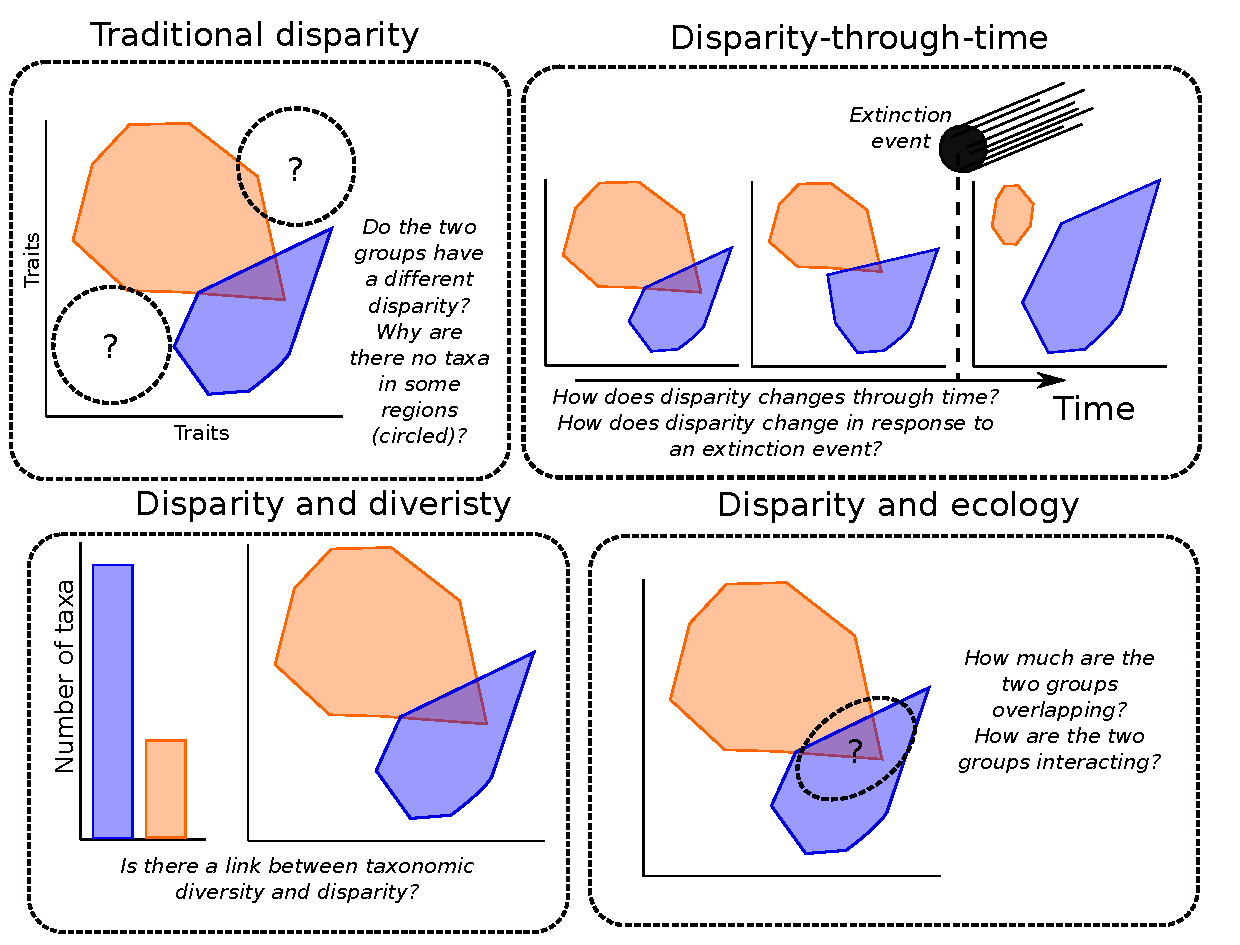
\includegraphics[width=0.9\textwidth]{Figures/figure_disparities.pdf}
% \caption{
%     The four main types of disparity analysis. \textbf{Descriptive disparity} focuses on describing the features of morphospace occupation; \textbf{\textcolor{blue}{disparity through time}} investigates the evolution of the morphospace through time including the effect of extinction events; \textbf{disparity and taxonomic diversity} compares different measures of biodiversity; \textbf{disparity as a proxy for ecology} uses disparity as a proxy for the ecological or functional role of a group.
%     These categories are not independent and many disparity studies will cover more than one.
% }
% \label{Fig:disparity}
% \end{figure}



\section{Data and disparity} \label{section:data}


\noindent Disparity analyses are based on traits, but traits can be characterised in a number of ways:
1) discrete morphological characters, e.g. coding the absence or presence of features or a discrete characteristic of a trait (e.g. \citealt{Foote1989, Deline2018});
2) continuous measurements of features (e.g. lengths in \citealt{Friedman2010});
or 3) more mathematical descriptors from geometric morphometric landmark data (e.g.
Procrustes coordinates)  (e.g. \citealt{sherratt2017rates}), Fourier coefficients (e.g. \citealt{Foote1995, Spriggs2018}) or model-based descriptors (e.g. \citealt{Raup1961,Saunders2004} - Fig. \ref{Fig:data}).
None of these approaches is superior, but they may be more or less well-suited to characterising the traits compared and to the question being asked using those traits \citep{hetherington2015cladistic,Hopkins2017}.

For example, if investigating variation of bat wing shapes, both homologous landmarks and continuous measurements of bones may be appropriate to capture patterns of wing variation.
If the question focuses on comparing wings between bats and birds, however, different measurements might be more appropriate depending on the specific question.
That is, if the focus is whether the aerodynamic properties of wings vary within bats or between bats and birds, the traits collected should reflect these aerodynamic properties (e.g. wingspan, aspect ratio, etc.).
However, if the focus is on convergence between different bats and birds, it would be preferable to use traits that have facilitated flight in both groups (e.g.
digit length, integumentary system, etc.).
Where there is any doubt about which traits to analyse, it may be preferable to use several different kinds of data for the same feature to determine whether they capture the same pattern of disparity.

The points above assume that researchers are collecting their own data for disparity analyses, but this is often not the case.
Discrete characters are commonly recycled from phylogenetic studies (e.g. \citealt{Brusatte2008,Close2015}).
This is an efficient approach to character sampling, but it may artifactually increase disparity between phylogenetically distinct groups, since phylogenetic characters are often collected to discriminate among groups.
This needs to be considered when interpreting results, especially \textcolor{blue}{as synapomorphies can lead to apparent shift or increase in disparity when new clade appear (especially if the character-state distribution is skewed towards a particular clade).}
Furthermore, many datasets are limited to subsets of anatomy that are at least implicit samples of overall anatomy, but explicit tests of this assumption have shown that different aspects of morphology can exhibit different patterns of disparity \citep{Hopkins2017}.
The influence of trait choice on resulting disparity patterns can be especially challenging where the available data has non-random missing anatomical parts, such as the absence of soft tissue in the fossil record \citep{Deline2018}.

Trait data suffer from the same shortcomings as most biological datasets -- data can be missing, non-overlapping, hierarchical, inapplicable, ambiguous, polymorphic, correlated, or there may be an insufficient sample size \citep{Palci2018}.
Biological phenomena such as allometry and sexual dimorphism may also influence trait data.
More mundanely, data collection is constrained by the time and money available, making collating a ``perfect'' dataset impossible.
Ultimately, disparity analyses are characterised by the data, and subsamples of the universe of possible data may not have the power to uncover the full patterns of disparity.
Therefore, trait data should be collected with the scientific question in mind, or the question asked should be tailored to the limits of the data available.

\begin{figure}[!htbp]
\centering
   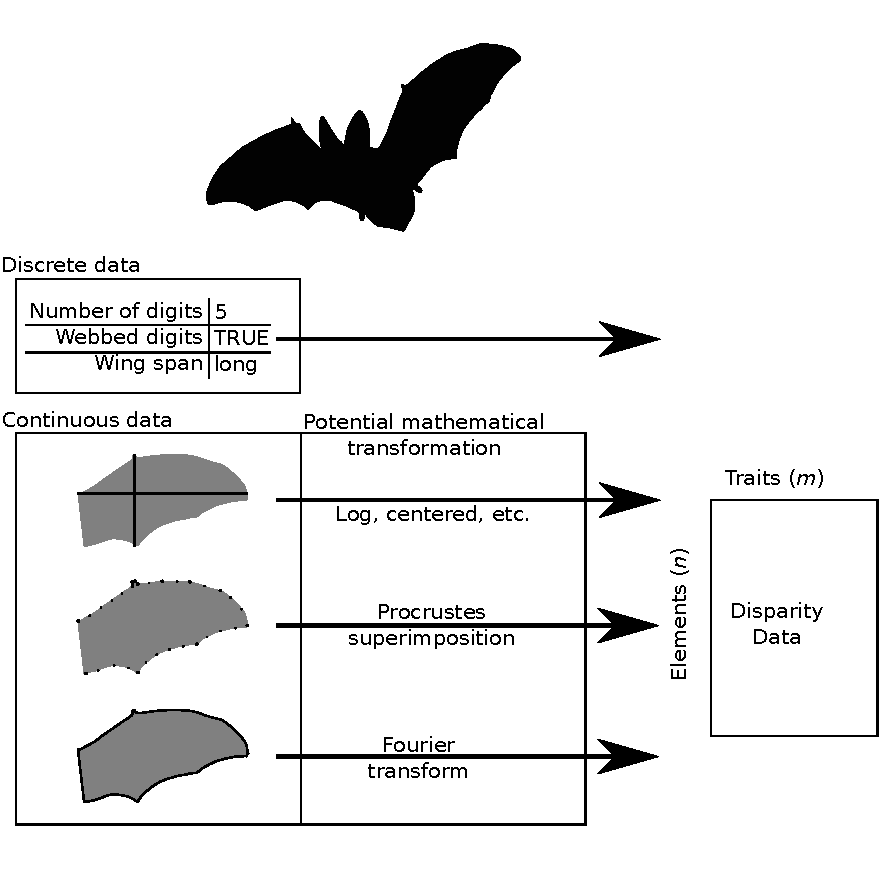
\includegraphics[width=0.9\textwidth]{Figures/figure_data.pdf}
\caption{
   Major routes to obtain morphological data for disparity analyses. Data can be collected as discrete trait observations (e.g. presence-absence data) or as continuous data. 
   Continuous data can be collected by various methods including linear measurements and landmark coordinates or contours (curves).
   These measurements can then be mathematically transformed (logarithmic transformations, scaling, Procrustes superimposition, elliptic Fourier transforms, etc.).
   Regardless of the method, data collection produces a trait matrix where the observed traits constitute columns and the studied elements (generally taxa or OTUs) the rows. 
}
\label{Fig:data}
\end{figure}

\section{Disparity analysis methods} \label{section:methods}

\noindent Once suitable trait data have been collected, the design of the disparity analysis itself needs to be considered.
Study design encompasses several key aspects including \ref{section:ordination} the difficulty of dealing with multidimensional data; \ref{section:metrics} the indices used to summarise the relative disparity of groups; \ref{section:testing} the methods used for hypothesis testing within the disparity analysis framework; and \ref{section:phylo} the influence of phylogeny on disparity analyses.
We consider these aspects in order below.

\subsection{To ordinate or not to ordinate - that is the (multidimensional) question} \label{section:ordination}

Disparity analyses often use ordination techniques for dimension reduction.
Ordinations are statistical methods that map observed variables onto a new space of reduced dimension while maintaining the requirement that similar observations are closer together than dissimilar ones (e.g. principal component analysis - PCA; principal coordinates analysis - PCO/PCoA; non-metric multidimensional scaling - NMDS).
They come in many flavours depending on the data and the desired morphospace properties.
For example, quantitative (continuous) data can be reduced using PCA, and qualitative data (\textcolor{blue}{or quantitative, or both}) can be reduced using PCO (which is equivalent to metric multidimensional scaling (MDS)) or non-metric multidimensional scaling (NMDS; see \citealt{Legendre2012} chapter 9 for a detailed overview of ordination methods and properties).
\textcolor{blue}{Note that when using a PCO, the distance metric on which to calculate the PCO can have some significant impact on the result morphospace} \citep{lehmann2019}.

One of the reasons why ordination techniques are common in disparity analysis is that they make it easier for researchers to comprehend patterns in two or three spatial dimensions at a time, which can be more intuitive than through disparity indices (see section \ref{section:metrics} below).
Additionally, after ordinating the data, it is possible to focus on just a subset of axes of the morphospace (i.e.
selecting only those axes that describe the majority of the variation in the dataset - e.g. 95\%).
In the case of geometric morphometric data, ordination is particularly useful as it conserves the mathematical properties of the data while efficiently reducing the dimensions \citep{Legendre2012,dryden2016statistical}.
In practice, this facilitates interpretation of only the major axis of a highly dimensional dataset as major gradients of biological variation (e.g. the elongation and flattening of birds beaks; \citealt{bright2016shapes}).

Like most other aspects of disparity analyses, however, reducing dimensionality can be fraught.
In the case of ordination, subsampling axes from the ordination can lead to misinterpretation of the results.
Although a common technique is to consider the \textit{d} axes that encompasses 95\% or 99\% of the variance in the dataset \textcolor{blue}{(either by manually selecting the \textit{d} axes that encompasses the desired variance or using methods such as the broken stick model; \citealt{Legendre2012} p.410)}, the interpretation of these principal axes can be unrepresentative of the data and lead to misinterpretation of the biological variation mapped on these axes \citep{Bookstein2015, Weisbecker2019}.
Visual interpretations of multidimensional data can be particularly misleading, not least as multidimensional spaces are not necessarily Euclidean even when analysing \textcolor{blue}{geometric} morphometric data \citep{Deline2018, Gerber2017}.

Interpreting biological variation along the axes is always a \textit{post-hoc} procedure and may have little relation to the overall question (for example, if the first few ordination axes represent elongation of the beak in birds, but the question is about wing disparity).
Additionally, in some cases, reducing the dimensionality of a dataset can render its interpretation more problematic.
For example, when the analysed data are non-Euclidean (e.g. some types of discrete morphological characters such as inapplicable characters), interpreting the resulting ordinated space can be challenging \citep{Gerber2019}.
This is problematic when comparing the position of groups in multidimensional space, as the distances might not be linear \textcolor{blue}{(although this can sometimes be corrected \citealt{cailliez1983})}.
Furthermore, \textit{post-hoc} interpretations of the gradient of variation on the ordination axes may be biologically meaningless or simply impossible \citep{Gerber2019}.
Although some gradients are easy to detect or interpret (e.g.
the elongation and depth of mandibles in fishes on first and second PC axes, respectively; \citealt{Hill2018}), some are not (e.g. \citealt{Weisbecker2019}).
For example, with discrete morphological data, a gradient between the species that have many characters in state 1 and those that have more in state 0 has no biological meaning if these are binary alternate states.

In general, categorical data are a good deal more problematic than continuous data, because the characters themselves are invariably non-equivalent, non-independent, and mostly non-Euclidean, and the distribution of the variance is usually more evenly distributed across axes (i.e. contrary to a PCA, the first few axes do not encompass most variance of the dataset).
Such non-Euclidean spaces often have non-intuitive properties, for example, straight lines viewed in bivariate plots of some dimensions are not actually straight and, character coding and missing data can make the pairwise dissimilarity matrix lose its metric properties (i.e. the distance between A and B is not equal to the distance between B and A; \citealt{Gerber2014}).
Last, but not least, in many cases, ordination might not be necessary.
For example, if an index characterising disparity can use all of the data, it is not necessary to calculate it on the ordinated dataset (e.g. \citealt{Close2015}).
For all of these reasons, multidimensional data should not be ordinated automatically, and careful consideration should be given to whether the aim of the study can be achieved without ordination \citep{lloyd2016,lloyd2018}.

\begin{figure}[!htbp]
\centering
   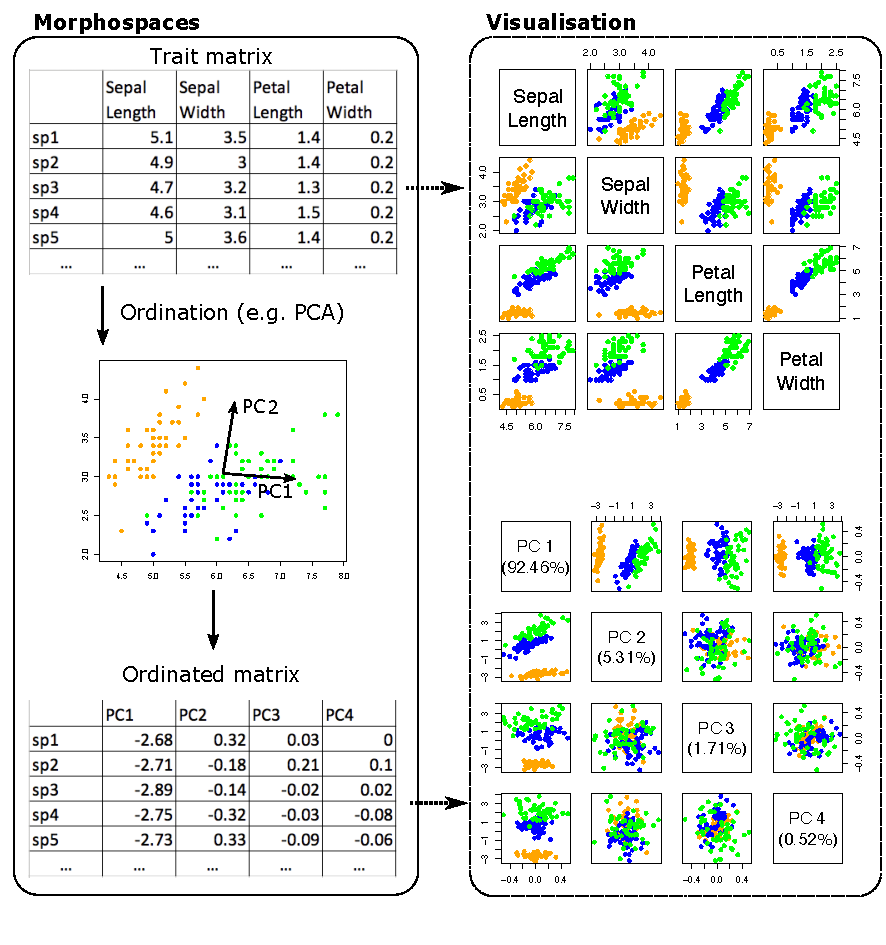
\includegraphics[width=0.9\textwidth]{Figures/figure_space2.pdf}
\caption{
    \textcolor{blue}{Illustration between the different morphospaces and visualisation of the same dataset (the classic ``iris'' dataset of} \citealt{edgar1935irises,fisher1936use}).
    \textcolor{blue}{Morphospaces: different mathematical representations of a morphospace. A trait matrix can be ordinated matrix (e.g. in }\citealt{tyler2011detecting}\textcolor{blue}{ - or transformed into a distance matrix }\citealt{Close2015}\textcolor{blue}{, not represented here).}
    \textcolor{blue}{Here we consider all these matrices as being \textit{morphospaces}, i.e. objects containing all the combinations of traits and observations (albeit transformed differently).
    Visualisation: different  ways to represent the morphospace in 2D.
    Visualisations can use either trait plots (directly from the trait matrix); or ordination axis plots (directly from the ordinated matrix).
    Note that in 2D representations, it is good practice to plot both axes on the same scale to avoid visually distorting the importance of one axis).}
}
\label{Fig:morphospace}
\end{figure}

\subsection{Measuring disparity} \label{section:metrics}

Most disparity datasets are multidimensional and, consequently, a large component of any disparity analysis involves considering how to extract a meaningful (i.e.
interpretable) summary of disparity.
This is usually achieved with a disparity measure or index \citep{Hopkins2017}.
As with any summary of multidimensional data, disparity indices will reflect only some aspects of the morphological variation, never its whole complexity \citep{GuillermeMOMS}.
It is therefore often beneficial to use more than one index to summarise different aspects of variation, guided by the aim of the study.

When considering only one dimension, \textcolor{blue}{disparity indices can be used compare the spread of the distributions (e.g. the range, quantiles or variance) or the differences in the central tendencies (i.e. mean, median or mode) of groups in the morphospace.}
Among these indices, some will have more attractive properties than others, such as sensitivity to outliers.
Range and mean are highly sensitive, whereas quantiles, variance and median are less so, making them more or less appropriate for different questions.
For example, if the goal is to characterise the extent of morphospace occupied by a group (e.g. does group A occupy as much space as group B?), indices related to the spread of the group in the morphospace are most appropriate (e.g.
volume; \citealt{Diaz2016}, distance from the centroid; \citealt{Hopkins2017, Finlay2015}, variance and range; \citealt{Brusatte2008}).
Furthermore, aspects other than variation (\textit{sensu} disparity) can be of interest: if we wish to describe the ``position'' of a group in a morphospace (e.g.
does group A occupy the same space as group B?), indices related to the distance between the elements within a group and a fixed point in the morphospace are most appropriate \citep{GuillermeMOMS}.
Finally, if we aim to characterise the density of morphospace occupation (e.g.
is group A more closely packed than group B?) indices related to the pairwise distances between elements will be most appropriate (e.g. nearest neighbour distance, pairwise distances, etc. \citealt{Close2015} - see section \ref{section:ordination} above).

In addition to considering which properties of disparity these indices capture, it is also important to consider the mathematical properties of the indices and their associated caveats \citep{Wills2001, Ciampaglio2001}.
For example, measuring the sum of variance for each dimension of the space is equivalent to measuring the sum of variance in a PCA (because the co-variance is null).
However, this is no longer true of other transformations of the space or when a subset of dimensions or elements are considered, such as is often done after PCA \citep{Legendre2012}.

Furthermore, multidimensional spaces have some counterintuitive properties that should be considered, such as the ``curse of dimensionality'' \citep{Bellman1966}.
In spaces with some axes of variance lower than one, product-based indices used as proxies of volumes (e.g. product of ranges, hypervolume, hypercube, etc.) can tend quickly tend towards zero for spaces with even a modest number of dimensions \citep{Bellman1966}.
Other types of indices are also extremely sensitive to outliers and can be biased easily by sample size, for example range \citep{Wills2001} or convex hull based \citep{Jackson2011} indices.

\subsection{Testing hypotheses about the evolution of disparity} \label{section:testing}

No matter which disparity indices have been calculated, the research question must be framed in an appropriate statistical context.
The multidimensional statistical toolkit for ecology and evolution has greatly expanded in recent years \citep{clavel2015mvmorph, Adams2018}, but some of these advances have yet to be implemented in disparity analyses.
Instead, hypothesis testing has been mostly confined to a small set of well-established methods.
One commonly used test is the non-parametric permutation analysis of variance (PERMANOVA) \citep{Anderson2001} that tests whether two groups share the same centroid and dispersion based on a distance matrix between observations.
\textcolor{blue}{The last decade has also seen a series of development based on this test (e.g. the linear regression for multidimensional data \citealt{collyer2015method} or the phylogenetic ANOVA \citealt{Adams2014}; but see \citealt{Adams2018,lloyd2016} for more).
It is worth noting that most of these test do not require the morphospace to be ordinated (see section \ref{section:ordination} above).
Regardless of the statistical test used, they should be employed that are tailored to the question at hand, rather than simply following common practices.}

It is also important to consider which data should be subjected to a statistical test.
For example, in morphological disparity analysis, especially for palaeobiological questions, data are often bootstrapped.
This has two advantages: (i) when the disparity index is unidimensional (e.g. the sum of variances), bootstrapping the data generates a distribution of the index that can be analysed using the vast statistical toolkit available for comparing distributions; (ii) when data are scarce, bootstrapping the data allows users to introduce variance, rendering the test less sensitive to outliers.
However, bootstrapped data are pseudoreplicates and thus non-independent \textcolor{blue}{and can increase the false positive rate (Type I error)} \citep{strube1988bootstrap}.
\textcolor{blue}{This, again, highlights the importance of tailoring the statistical test to the data and question at hand.}

Finally, it is important to understand the limitations of the dataset for performing statistical analysis.
Mainly, disparity analysis should be restrained to groups within the same morphospace and are more difficult between different morphospaces.
This can be the case when comparing elements with different numbers of landmarks or different landmark configurations which will result in different morphospaces;comparing disparity indices between these is not trivial.

\subsection{Disparity and phylogeny} \label{section:phylo}

As with all comparative datasets, the data used in disparity analyses are not independent because close relatives will tend to have more similar morphologies than more distant relatives \citep{Harvey1998}.
Thus, for disparity analyses that consider groups with phylogenetic relationships (which is common), the non-independence between observations should be taken into account.
It has been noted, however, that some popular phylogenetic correction methods (like phylogenetic PCA) can be inappropriate, especially when using only the first \textit{d} axis of the ordination, and can lead to incorrect interpretations of the data (such as wrongly supporting ``early burst'' type patterns; \citealt{Uyeda2015}).
\textcolor{blue}{Furthermore, phylogenetic PCA are also really dependent on the evolutionary model which can be sometimes difficult to choose (e.g. the default Brownian motion model is not always appropriate;} \citealt{blomberg2020}).

One other common way to take phylogeny into account in disparity analyses is using ancestral state estimations in \textcolor{blue}{disparity through time} analyses to extract disparity estimates for non-sampled taxa and/or nodes of a phylogeny \citep{brusatte2011phylogenetic,Guillerme2018}.
Ancestral state estimation can be performed at two points in the disparity analysis pipeline: either (1) pre-transformation, i.e. the estimation is done before transformation of the data (e.g. ordination, or distance matrix construction) and is simply based on the original data; or (2) post-transformation, i.e. the estimation is done after transformation of the data by estimating the ancestral states using the transformed matrix (e.g. the ordination scores; \citealt{lloyd2018}).

Pre-transformation ancestral state estimation will change the way the ordination space is defined -- i.e.
the relationship between the points is not yet estimated -- and requires longer computational times.
However, once the morphospace is defined, its properties will not change.
Post-transformation ancestral state estimation will not change the empirical ordination space and is faster to compute, but it will add elements in the space, whose estimated positions can be problematic for statistical tests and evolutionary inferences down the line \citep{lloyd2018}.

All ancestral state estimates are highly dependent on the data and method used \textcolor{blue}{(especially which evolutionary model)} \cite{louca2020}.
In general, using ancestral state estimation can help with recovering patterns of change in disparity but should not be used simply to generate extra data points to increase statistical power.
In fact, these extra points are not independent and can also have problematic side effects, especially when testing for the influence of mass extinctions on disparity as they artificially and asymmetrically increase taxon sampling.

\section{Disparity analyses for the future} \label{section:future}

\noindent Morphological disparity analyses are widely employed in evolutionary palaeobiology, and are based on a diversity of methods and data.
There is no ``one-size-fits-all'' pipeline for morphological disparity analyses.
As with any multidimensional analysis, there are many variables that have to be considered when deciding which data to use and how to analyse them, stemming from the explicit hypotheses being tested.
Although this makes comparison between disparity analyses difficult and makes generalisation required to answer the general biological questions from the introduction still premature (e.g. how does phenotypic variation evolves?), this diversity of methodological approaches provides researchers with a great number of tools tailored to answer specific biological questions.

Many of the problems in morphological disparity analysis arise from ``blind'' application of established methodological pipelines without consideration of the biological question being addressed.
We advocate that researchers should assemble their analytical protocol based on an experimental approach that explores the impact of competing methods, such as choice of indices, ordination method, and ancestral state estimation method on disparity analysis results.
Thankfully, this is becoming easier through the availability of diverse, well documented R packages for multidimensional analysis \citep{Bouxin2005, oksanen2007vegan, Harmon2008, lloyd2016, Guillerme2018b}.
Many of the methods employed in disparity analysis are used more widely in other fields, including genomics and ecology, which also encompass analyses of multidimensional datasets \citep{Donohue2013, Saupe2015, Canter2018, mammola2019}.
Innovations in morphological disparity analyses likely await discovery in their respective literatures.

While studies of morphological disparity would benefit from advances in multidimensional analysis in other fields, the concept of a morphospace could reciprocally benefit other disciplines.
For example, the multidimensional analysis of \citep{Diaz2016}, which analysed patterns of form and function in plants, is essentially an eco-morphospace; isotopic analyses of organisms \citep{Jackson2011,Swanson2015} can be represented as an isotope-space; ecosystem functioning in \citealt{Donohue2013} as an ecosystem-space \citep{qiao2017}, etc.
These generalisations could also be exported for any set of traits: cognate approaches have been adopted in the analysis of single cell comparative transcriptome data \citep{Sebe-Pedros2018} where interpretation of the resulting transcriptome-spaces would be improved by giving careful attention to the concerns we highlight concerning morphospaces.

Although disparity analyses are now simple to implement in freely available software \citep{Bouxin2005, oksanen2007vegan, Harmon2008, lloyd2016, Guillerme2018b} it is crucial to remember that they are multidimensional analyses and that multidimensional analyses are complex.
We assert that future morphological analyses will benefit from emphasising the methodological decisions made, rather than simply using disparity analysis because it exists.

\subsection{Author contributions}

TG, NC and PD proposed this review; TG and NC led the writing supported by PD and GT.
All authors edited drafts and approved the final version.

\subsection{Acknowledgements}

This article results from discussion at the Royal Society International Science Seminar on `Reconciling disparate views on disparity' held at Chicheley Hall, 9-10th January, 2018.
\textcolor{blue}{We thank the two anonymous reviewers for their helpful and positive comments.}
AG was funded by European Research Council Starting grant 637171 ADaPTiVE;
ALJ was funded by an Irish Research Council Laureate Award IRCLA/2017/186;
ES was funded by a University of Adelaide Research Fellowship;
EES was funded by a Leverhulme Trust Research Project Grant (DGR01020);
PD was funded by NERC (NE/P013678/1; NE/N002067/1) and BBSRC (BB/N000919/1);
SB was funded by European Research Council (ERC) under the European Union's Horizon 2020 research and innovation program (grant agreement No 756226, ERC Starting Grant: PalM) and a Leverhulme Trust Research Project Grant (RPG-2017-167);
TG was funded by ARC DP170103227 and FT180100634 awarded to VW;
GHT was funded by European Research Council Consolidator Grant 615709 ToLERates and Royal Society University Research Fellowship UF120016.

\bibliographystyle{sysbio}
\bibliography{References}

\end{document}

